\section{Checkpoint 4 - Memory Management}

% align with slide numbers
\addtocounter{subsection}{1}

\subsection{\important What is the role of the Memory Management Unit (MMU)}
Sie übersetzt logische (Adresse im Programm) auf physikalische Adressen (Adresse auf Festplatte).
(Passiert bei jedem Speicherzugriff neu.)

\subsection{\important What is the difference between virtual / logical Adresses and physical adresses?}
Der physische Bereich existiert genau ein mal.
Seine Größe ist abhängig von der Anzahl der Module.\\
Es gibt einen virtuelle Bereich für jeden Prozess.
Diese sind eine Abbildung auf den physikalischen Bereich.
Seine Größe ist abhängig von der Anzahl der Adressen.

\subsection{What is Segmentation?}
Einteilung des Speichers in abgeschlossene Segmente.
Ein Segment ist charakterisiert durch seine Startadresse und seine Größe.
Sie sind Speicherreservierungen für einzelne Prozesse.
Damit können wir sichergehen, dass ein Speicherzugriff eines Prozesses immer in seinem Segment landet.

\subsection{What are the main shortcommings of Segmentation?}
externe Fragmentierung: Prozesse terminieren und ihr Speichersegment wird freigegeben. Damit entstehen aber Löcher zwischen Segmenten, die eventuell nicht gefüllt werden können.\\
interne Fragmentierung: Ein Prozess nutzt nicht das gesamte Segment, das er reserviert hat.\\
sehr unflexibel in Speichergröße: Häufig wird deswegen mehr Speicher reserviert, was aber zu mehr Fragmentierung führt.\\
Anzahl der Prozesse ist limitiert durch die Größe der reservierten Speicher.

\subsection{Describe Paging. \important How is it different from Segmentation, and how does it address the shortcumings of Segmentation?}
Ein Prozess kann mehrere Speicherbereiche (Pages) haben.
(Anders als bei Segmentation.)
Die Anzahl der Pages ist dabei dynamisch, also zur Laufzeit, festgelegt.\\
Damit gibt es keine externe Fragmentierung mehr, da Löscher zwischen den Pages wieder mit neuen Pages aufgefüllt werden können und es gibt weniger interne Fragmentierung da die Pages kleiner sind und wir uns bei Bedarf neue Pages dazu holen können.
Da Pages ausgelagert werden können, ist die Anzahl der Prozesse auch nicht mehr limitiert.\\
(Page) Frame: ein physischer Speicherblock\\
page: ein virtueller Speicherblock; manchmal wird der Begriff auch für beides verwendet.

\subsection{Describe the layout of a Page Table.}
Eine Tabelle welche virtuelle Speicherbereiche auf physische Speicherbereiche abbildet.
Eine Page Table ist zur Laufzeit veränderbar und wird von der MMU genutzt.
In der Praxis ist es nur eine Liste mit physichen Page Frame (Nummern), und die virtuelle Page (Nummer) ist der Index.

\subsubsection{Why do some architectures use multi-level page table structures?}
Um Speicherplatz zu sparen, da eine Page Table sehr groß ist. Damit müssen wir nur die Page Table Einträge wirklich ausfüllen, welche wir auch verwenden.
(Beispiel: Bei Intel 64-Bit Systemen gibt es vier Ebenen an Page Tables.)

\subsection{\important Name two bits associated with each Page Table Entry and describe their purpose.}
Dirty: wurde auf die Page geschrieben? Wenn ja, müssen wir sie abspeichern, bevor wir sie wegwerfen.\\
Read/Write/Execute: Berechtigungsbits\\
Valid: wenn die Page eine gültige Abbildung im physikalischen Speicher hat. (Wenn das Valid Bit nicht gesetzt ist, darf auf die Page nicht zugegriffen werden.)\\
(\todo Weitere siehe Folien)

\subsection{What is the role of the Translation Lookaside Buffer (TLB)?}
Es ist ein Cache für Seitenzugriffe: Es speichert kürzlich erfolgte Umwandlungen von virtuellen in physische Adressen.
Damit sparen wir uns das Nachsehen in diversen Page Tables, wenn wir einen Cache Hit haben.
Bei einem Miss wird das Ergebnis der Umwandlung der MMU in die TLB eingetragen.
Es funktioniert mit Registern und ist entsprechend sehr schnell.

\subsection{Assume a memory system that manages adresses of 26 bits length, with a page size of 256 bytes.}
\textit{Die Reihenfolge wurde leicht geändert.}
\subsubsection{What is the size of the virtual adress space?}
Adresslänge: $26 \Bit$\\
Größe des virtuellen Addressraumes (entspricht Anzahl aller möglichen Adressen): $2^{26} \Byte = 2^6 * 2^{20} \Byte = 64 \MiB$

\subsubsection{How long are the adresses' page number and offset?}
Page Size: $256 \Byte = 2^8 \Byte$\\
$\Rightarrow$ Offset Länge (entspricht der Anzahl an Bits die wir benötigen, um alle Adressen in einer Page zu bilden): $8 \Bit$\\
Page Number Länge (Die verbleibenden Bits können dann für das Adressieren der Page Nummer in der Page Table genutzt werden.): $26\Bit - 8\Bit = 18\Bit$

\subsubsection{How many entries does a page table have?}
Annahme: Single Level Page Table\\
Anzahl der Einträge in der Page Table (entspricht der Anzahl der Adressen die mit der Page Number Länge gebildet werden können): $2^{18}$ 

\addtocounter{subsection}{2}
\subsection{\textit{Same as above.} Each page table entry has two status bits.}
\subsubsection{What is the length of a page table entry?}
Annahme: Addresslänge einer virtuellen Adresse ist identisch zur Adresslänge einer physischen Adresse.\\
Länge eines Page Table Eintrags: $18\Bit + 2\Bit = 20\Bit$

\subsubsection{What is the total size of a page table?}
\textit{Es kann auch sein, dass ein Eintrag auf Wort Länge (ist meist Addresslänge, also hier 26 Bit) aufgerundet wird. Hier ist das aber nicht der Fall.}\\
Gesamtgröße (ist Länge eines Eintrages * Anzahl der Einträge):
$$
\begin{aligned}
    2^{18} * 20\Bit &= 2^3 * 2^{15} * 20 \Bit\\
    &= 2^{15} * 20 \Byte\\
    &= 2^{10} * 2^5 * 20 \Byte\\
    &= 2^{10} * 2^6 * 10 \Byte\\
    &= 2^6 * 10 \KiB\\
    &= 640 \KiB
\end{aligned}
$$
Zum Vergleich, wenn auf Addresslänge aufgerundet wird: $832 \KiB$\\
Wenn auf Bytelänge (also 24) aufgerunder wird: $768 \KiB$

\subsection{Assume the described system has access to 24MiB of physical memory, half of which is reserved for the operating system. Of this half, 5MiB are reserved for process page tables, and are not pageable. How many processes can this system support?}
Aufteilung ist also: $5 \MiB$ für Page Tables, $7 \MiB$ für andere Dinge vom Betriebssystem, $12 \MiB$ für Prozesse.\\
Da jeder Prozess eine eigene Page Table hat, schauen wir, wie viele Page Tables wir in diese $5 \MiB$ kriegen:
$$
\begin{aligned}
    5 \MiB / 640 \KiB &= 5 * 2^{10} \KiB / 640 \KiB\\
    &= 5 * 2^{10} / 640\\
    &= 2^{10} / 128\\
    &= 2^{10} / 2^7\\
    &= 2^3 = 8
\end{aligned}
$$
\textit{Bei einer ungeraden Zahl müssen wir logischerweise abrunden.}

\subsection{What is the maximum size of a process working set, assuming that no reserved OS pages are part of the working set (\ref{WorkingSet})?}
Ein Prozess kann maximal $12 \MiB$ an Speicher reserviert haben.

\subsection{\important What is a Page Fault?}
Zugriff auf eine Page auf der das Valid Bit nicht gesetzt ist. Ein Page Fault löst wiederum einen Interrupt aus.

\subsection{What is the difference between a Soft Page Fault and a Hard Page Fault?}
Soft Page Fault: Die Page bedindet sich noch im Cache und kann noch leicht zurück geholt werden.\\
Hard Page Fault: Die Page muss komplett neu in den Hauptspeicher (von der Platte) geladen werden.

\subsection{Name two different reasons for which a memory access coul produce a Page Fault.}
Daten sind bereits ausgelagert und befinden sich nicht mehr im Hauptspeicher, Wir schreiben auf eine Copy-On-Write Page, Zugriff auf reservierten aber nicht committeden Speicher (\ref{ResCom}), wir greifen auf eine Page zu, auf die wir keine Berechtigung haben, wir greifen auf Speicher zu an dem sich noch keine Page befindet

\subsection{\important What is a Working Set?\label{WorkingSet}}
Menge aller Hauptspeicherseiten auf die ein Prozess zugreifen kann, ohne ein Page Fault zu erzeugen.

\subsection{What is the role of the Modified, Standby, Free, Zero and Bad Page Lists?}
Die Listen ergänzen die Working Sets der Prozesse um eine genauere Einteilung der Pages zu ermöglichen.

\subsubsection{What properties do pages in these lists have?}
\begin{itemize}
    \item[Modified:] Seiten die noch zu einem Prozess gehören, bei denen aber das Dirty Bit gesetzt ist
    \item[Standby:] ähnlich, nur ist das Dirty Bit hier nicht gesetzt
    \item[Free:] Seiten die zu keinem Prozess gehören, aber noch Restdaten enthalten
    \item[Zero:] komplett genullte Seiten
    \item[Bad:] defekte Seiten, werden vom System zur Boot Zeit beim Memory Check erkannt
\end{itemize}

\subsubsection{How do pages transition between these lists?}
\begin{figure}[H]
	\centering
	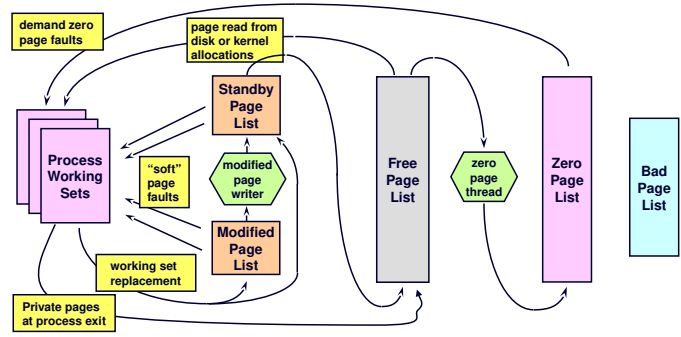
\includegraphics[width=0.7\linewidth]{Pictures/PageLists}
\end{figure}

Free nach Zero: Zero Page Thread (wird gemacht sobald Zeit ist; muss aber nicht gemacht werden, wenn die Seite sowieso überschrieben wird, zum Beispiel beim Laden einer Binary)\\
Working Set nach Modified / Standby: Balance Set Manager Thread, falls das System den Speicher für andere Prozesse braucht, oder falls Speicher lange nicht mehr genutzt wurde\\
Modified nach Standby: sobald Änderungen gesichert wurden\\
Working Set / Modified / Standby nach Free: wenn Prozess terminiert

\subsection{What is the purpose of the Page Frame Number Database?}
Struktur bei der für jede physikalische Page Frame ein Eintrag existiert.

\subsection{\important Describe the page replacement algorithms First-In-First-Out (FIFO), Second Chance, and Least-Recently-Used (LRU).}
Page replacement: wenn eine Page aus dem Working Set in die Modfied / Standby List verschoben wird.\\
\begin{itemize}
    \item[FIFO:] Die alteste Page Frame wird ausgelagert
    \item[Second Chance:] FIFO über alle Seiten, die (seit dem letzten Page replacement) nicht verwendet wurden (in der Regel besser als FIFO)
    \item[LRU:] Die am längsten nicht verwendete Page wird ausgelagert (die teuerste Methode von allen)
\end{itemize}

\subsection{What is Béládys Anomaly, as found in the FIFO page replacement algoritm?}
Mehr physikalische Pages können dazu führen, dass FIFO replacement schlechter funktioniert.

\subsection{Assuming three frames of physical memory, and a memory access pattern to the virtual pages: 2,1,4,2,3,4,2,1,3,4,3. How many Page Fault would FIFO incur?}
\begin{tabular}{c|ccccccccccc}
    &2&1&4&2&3&4&2&1&3&4&3\\
    \hline
    1.&\underline{2}&2&2&\textbf{2}&\underline{3}&3&3&3&\textbf{3}&\underline{4}&4\\
    2.& &\underline{1}&1&1&1&1&\underline{2}&2&2&2&\underline{3}\\
    3.& & &\underline{4}&4&4&\textbf{4}&4&\underline{1}&1&1&1
\end{tabular}
\\
Unterstriche: Page Fault; Fett: Page Hit\\
Insgesamt 8 Page Faults (5 ohne die initialen)

\subsection{How many Page Faults would Second Chance incur?}
\begin{tabular}{c|ccccccccccc}
      &2&1&4&2&3&4&2&1&3&4&3\\
    \hline
    1.&\underline{2}&2&2&\textbf{2}&2&2&\textbf{2}&2&\underline{3}&3&\textbf{3}\\
    2.& &\underline{1}&1&1&\underline{3}&3&3&\underline{1}&1&1&1\\
    3.& & &\underline{4}&4&4&\textbf{4}&4&4&4&\textbf{4}&4
\end{tabular}
\\
Fett: Access Bit wird gesetzt\\
Insgesamt 6 Page Faults.

\subsection{How many Page Faults would LRU incur?}
\begin{tabular}{c|ccccccccccc}
    &2&1&4&2&3&4&2&1&3&4&3\\
  \hline
  1.&\underline{2}&2&2&\textbf{2}&2&2&\textbf{2}&2&2&\underline{4}&4\\
  2.& &\underline{1}&1&1&\underline{3}&3&3&\underline{1}&1&1&1\\
  3.& & &\underline{4}&4&4&\textbf{4}&4&4&\underline{3}&3&\textbf{3}
\end{tabular}
\\
Fett: Page Hit\\
Insgesamt 7 Page Faults.

\subsection{What is the difference between swapping and page replacement (paging)?}
Swapping bedeutet eigentlich das gesamte Segment eines Prozesses auszulagern. (Damit ist der Prozess effektiv nicht mehr lauffähig.)
Heute werden beide Begriffe für das gleiche Prinzip (page replacement) verwendet.
Page replacement ist das auslagern einzelner (selten benötigter) Pages.

\subsection{Describe the difference between reserved and committed memory.\label{ResCom}}
Reservierter Speicher ist der als verwendbar markierte \underline{virtuelle} Speicher.
Committed Speicher ist der einem Prozess zur Verfügung stehende \underline{physikalische} Speicher. 

\subsection{What is a Guard Page? What could it be used for?}
Eine Page welche das Ende eines Buffers (Arrays) markiert und dafür sorgt, dass ein Interrupt erzeugt wird, sobald auf die Guard Page zugegriffen wird und in diesem Interrupt wird dann der Buffer um eine weitere Page verlängert (eine weitere Page committed), an dessen Ende wieder eine Guard Page steht.
Eine Guard Page kann genutzt werden um Zugriff auf nicht reservierten Speicher oder Stack Overflows zu verhindern.

\subsection{How do operating systems implement shared memory?}
Ein Eintrag in der Page Table von zwei Prozessen zeigt auf die gleiche (physikalische) Page Frame.

\subsection{\important What is Copy-on-Write (CoW) memory, and what is it used for?}
Bei einem fork eines Prozesses, wird der Speicher in beiden Prozessen als CoW markiert.
Die physikalische Page Frame ist dabei identisch.
Sobald ein Prozess dann aber in diesen geteielten Speicher schreiben will, wird er kopiert, damit jeder Prozess seinen eigenen (unabhängigen) Speicher hat.
Damit sparen wir uns das Kopieren von Speicher, den wir vielleicht nie verändern.
